\documentclass[12pt,twoside,english,a4paper]{article}

\usepackage[english]{babel}
\usepackage[IL2]{fontenc} % lepšia sadzba písmena Ľ než v T1
\usepackage[utf8]{inputenc}
\usepackage{graphicx}
\usepackage{url} % príkaz \url na formátovanie URL
\usepackage{hyperref} % odkazy v texte budú aktívne (pri niektorých triedach dokumentov spôsobuje posun textu)

\usepackage{cite}
%\usepackage{times}

\pagestyle{headings}

\title\textbf{FOOTBAL SIMULATORS (FIFA AND PES)}

\author{Dmytro Barninets\\[2pt]
	{\small Slovenská technická univerzita v Bratislave}\\
	{\small Fakulta informatiky a informačných technológií}\\
	{\large \texttt{xbarninets@stuba.sk}}
	}

\date{\large 11. october 2022}



\begin{document}

\maketitle


\section{WHY DID I CHOSE THIS TOPIC?} \label{fifa}

The main reason I chose this theme is the popularity of football games. Among sports simulators, it is FIFA that occupies a leading position in online.


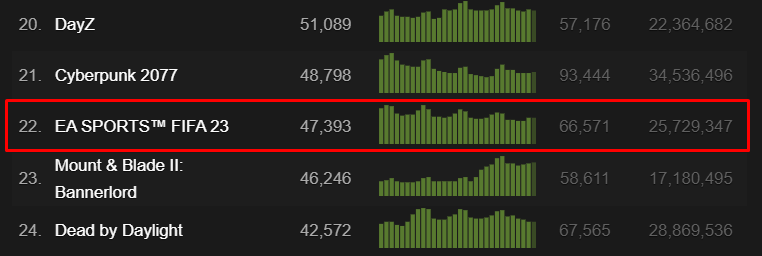
\includegraphics[width=150mm,scale=1.5]{fifa_charts.png} \label{foto}


As of November 4, an average of 47,000 players play FIFA. And this is only in Steam, excluding consoles and less popular game launchers.


As for PES, the situation with online is much worse at the moment \emph{(more on that later)}. But that doesn't stop footsim fans from remembering this series as legendary.

In general, football simulators are not as simple and monotonous as at first glance.

\section{Nejaká časť} \label{nejaka}

Z obr.~\ref{f:rozhod} je všetko jasné. 

\begin{figure*}[tbh]
\centering

Aj text môže byť prezentovaný ako obrázok. Stane sa z neho označný plávajúci objekt. Po vytvorení diagramu zrušte znak \texttt{\%} pred príkazom \verb|\includegraphics| označte tento riadok ako komentár (tiež pomocou znaku \texttt{\%}).
\caption{Rozhodujúci argument.}
\label{f:rozhod}
\end{figure*}



\section{Iná časť} \label{ina}

Základným problémom je teda\ldots{} Najprv sa pozrieme na nejaké vysvetlenie (časť~\ref{ina:nejake}), a potom na ešte nejaké (časť~\ref{ina:nejake}).\footnote{Niekedy môžete potrebovať aj poznámku pod čiarou.}

Môže sa zdať, že problém vlastne nejestvuje\cite{Coplien:MPD}, ale bolo dokázané, že to tak nie je~\cite{Czarnecki:Staged, Czarnecki:Progress}. Napriek tomu, aj dnes na webe narazíme na všelijaké pochybné názory\cite{PLP-Framework}. Dôležité veci možno \emph{zdôrazniť kurzívou}.


\subsection{Nejaké vysvetlenie} \label{ina:nejake}

Niekedy treba uviesť zoznam:

\begin{itemize}
\item jedna vec
\item druhá vec
	\begin{itemize}
	\item x
	\item y
	\end{itemize}
\end{itemize}

Ten istý zoznam, len číslovaný:

\begin{enumerate}
\item jedna vec
\item druhá vec
	\begin{enumerate}
	\item x
	\item y
	\end{enumerate}
\end{enumerate}


\bibliography{literatura}
\bibliographystyle{plain}
\end{document}
